\documentclass{article}

\usepackage{qa}

\begin{document}
\customtitle{Homework 5}
\customauthor{Hamza Kamal}
\customdate{\today}

\qna {
     1. Consider the logic gate circuit shown below (5 points) \\
     \begin{figure}[H]
          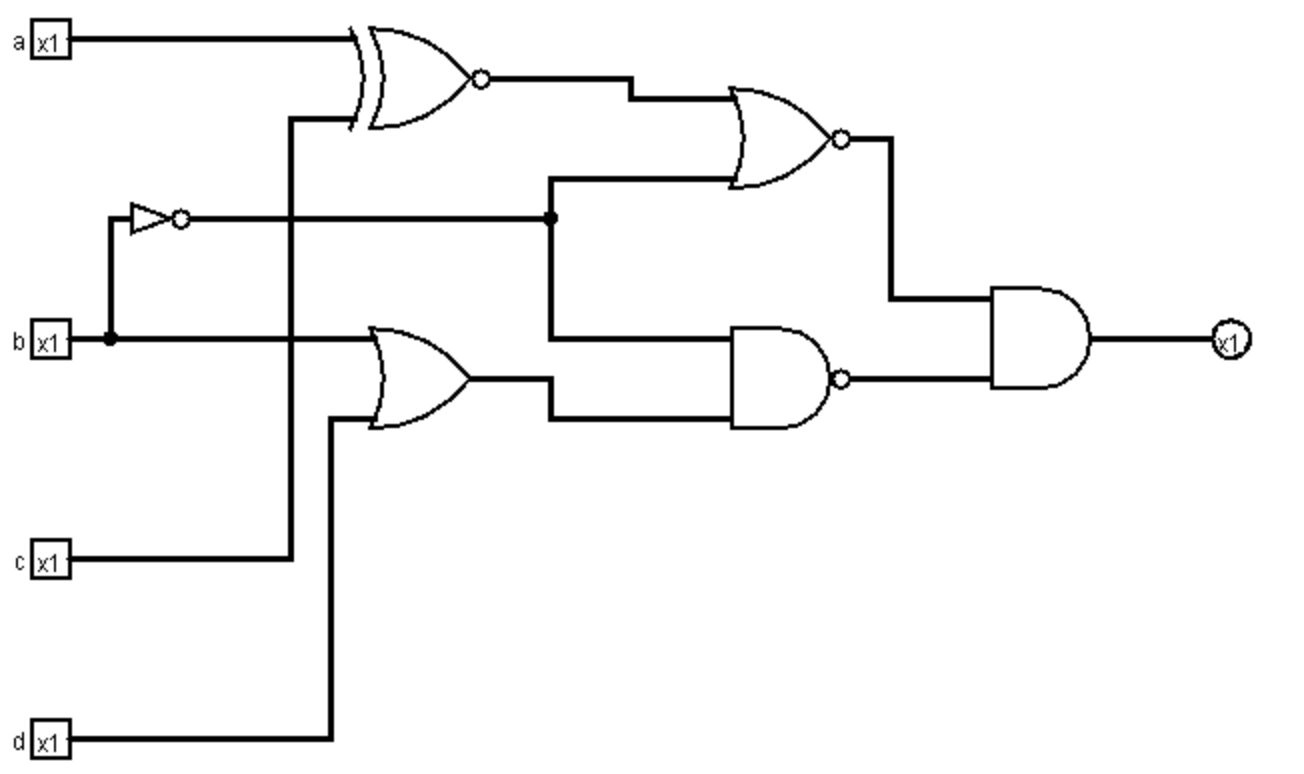
\includegraphics[width=\textwidth]{./img/circuit.png} 
     \end{figure}
     a. (2 points) Derive a Boolean equation for the output X. You don't need to simplify this equation, but feel free to try! \\
} {
     The first gate, which is an XNOR gate with the inputs \(a\) and \(c\), gives us: \\
     \(\neg(a \oplus c)\) \\
     \linebreak
     The second gate is an OR gate with inputs \(b\) and \(d\), which gives us: \\
     \(b \lor d\) \\
     \linebreak
     The third gate is a NOR gate with the inputs \(\neg(a \oplus c)\) and \(\neg b\), which gives us: \\
     \(\overline{\neg(a \oplus c) \lor \neg b}\) \\
     \linebreak
     The fourth gate is a NAND gate with the inputs \(\neg b\) and \(b \lor d\), which gives us: \\
     \(\overline{(\neg b) \land (b \lor d)}\) \\
     \linebreak
     The fifth gate is an AND gate with the inputs \(\overline{\neg(a \oplus c) \lor \neg b}\) and \(\overline{(\neg b) \land (b \lor d)}\), which gives us the final equation: \\
     \(\overline{\neg(a \oplus c) \lor \neg b} \land \overline{(\neg b) \land (b \lor d)}\)
}
\qna {
     b. (3 points) Draw a truth table for the circuit. \\
} {
     Truth Table: \\
     \begin{tabular}{|c | c | c | c | c|}
          \hline
          a & b & c & d & x \\
          \hline
          0 & 0 & 0 & 0 & 0 \\
          \hline
          0 & 0 & 0 & 1 & 0 \\
          \hline
          0 & 0 & 1 & 0 & 0 \\
          \hline
          0 & 0 & 1 & 1 & 0 \\
          \hline
          0 & 1 & 0 & 0 & 1 \\
          \hline
          0 & 1 & 0 & 1 & 1 \\
          \hline
          0 & 1 & 1 & 0 & 1 \\
          \hline
          0 & 1 & 1 & 1 & 1 \\
          \hline
          1 & 0 & 0 & 0 & 0 \\
          \hline
          1 & 0 & 0 & 1 & 0 \\
          \hline
          1 & 0 & 1 & 0 & 0 \\
          \hline
          1 & 0 & 1 & 1 & 0 \\
          \hline
          1 & 1 & 0 & 0 & 1 \\
          \hline
          1 & 1 & 0 & 1 & 1 \\
          \hline
          1 & 1 & 1 & 0 & 1 \\
          \hline
          1 & 1 & 1 & 1 & 1 \\
          \hline
     \end{tabular}
}

\qna {
     3. (14 points) Design a combinational circuit system. \\
     Design a combinational circuit with three inputs x,y,z, and three outputs A,B,C. When the binary inputs is 0,1,2,or 3, the binary output is two greater than the input. When the binary input is 4,5,6,or 7, the binary output is one less than the input. \\
     Please answer all of the following sub-questions. \\
     a. (3 points) x,y,z are inputs and A,B,C are outputs. Draw a truth table for the given function. \\
} {
     Truth Table: \\
     \begin{tabular}{| c | c | c | c | c | c | c | c |}
          \hline
          x & y & z & decimal & A & B & C & decimal \\
          \hline
          0 & 0 & 0 & 0 & 0 & 1 & 0 & 2 \\
          \hline
          0 & 0 & 1 & 1 & 0 & 1 & 1 & 3 \\
          \hline
          0 & 1 & 0 & 2 & 1 & 0 & 0 & 4 \\
          \hline
          0 & 1 & 1 & 3 & 1 & 0 & 1 & 5 \\
          \hline
          1 & 0 & 0 & 4 & 0 & 1 & 1 & 3 \\
          \hline
          1 & 0 & 1 & 5 & 1 & 0 & 0 & 4 \\
          \hline
          1 & 1 & 0 & 6 & 1 & 0 & 1 & 5 \\
          \hline
          1 & 1 & 1 & 7 & 1 & 1 & 0 & 6 \\
          \hline
     \end{tabular}
}

\qna {
     b. (3 points) Based on the truth table you draw, build Karnaugh maps for the output A,B,C. \\
} {
     Karnaugh Map for A: \\
     \begin{tabular}{| c | c | c | c | c |}
          \hline
          yz/x & 00 & 01 & 11 & 10 \\
          \hline
          0 & 0 & 0 & 1 & 1 \\
          \hline
          1 & 0 & 1 & 1 & 1 \\
          \hline
     \end{tabular} \\
     \linebreak
     Karnaugh Map for B: \\
     \begin{tabular}{| c | c | c | c | c |}
          \hline
          yz/x & 00 & 01 & 11 & 10 \\
          \hline
          0 & 1 & 1 & 0 & 0 \\
          \hline
          1 & 1 & 0 & 1 & 0 \\
          \hline
     \end{tabular} \\
     \linebreak
     Karnaugh Map for C: \\
     \begin{tabular}{| c | c | c | c | c |}
          \hline
          yz/x & 00 & 01 & 11 & 10 \\
          \hline
          0 & 0 & 1 & 1 & 0 \\
          \hline
          1 & 1 & 0 & 0 & 1 \\
          \hline
     \end{tabular}
}

\qna {
     (3 points) Derive (as simple as possible) Boolean equations for A,B,C using the Karnaugh maps \\
} {
     Boolean equation for A: \\
     Looking at the Karnaugh map: \\
     \begin{tabular}{| c | c | c | c | c |}
          \hline
          yz/x & 00 & 01 & 11 & 10 \\
          \hline
          0 & 0 & 0 & 1 & 1 \\
          \hline
          1 & 0 & 1 & 1 & 1 \\
          \hline
     \end{tabular} \\
     \linebreak
     We can create groupings for the 1's.\\
     The first group of 4 1's $(011, 010, 111, 110)$ gives us the equation: \\
     $A = y$ \\
     The second group of 2 1's $(101, 111)$ gives us the equation: \\
     $A = xz$ \\
     This gives us the final equation: \\
     $A = y \lor xz$ \\
     \linebreak
     Boolean Equation for B: \\
     Looking at the Karnaugh map: \\
     \begin{tabular}{| c | c | c | c | c |}
          \hline
          yz/x & 00 & 01 & 11 & 10 \\
          \hline
          0 & 1 & 1 & 0 & 0 \\
          \hline
          1 & 1 & 0 & 1 & 0 \\
          \hline
     \end{tabular} \\
     \linebreak
     We can create groupings for the 1's. \\
     The first group of 2 1's $(000, 001)$ gives us the equation: \\
     $B = \neg x \neg y$ \\
     The second group of 2 1's $(000, 100)$ gives us the equation: \\
     $B = \neg y \neg z$ \\
     The remaining 1 gives us the equation: \\
     $B = xyz$ \\
     This gives us the final equation: \\
     $B = (\neg x \neg y) \lor (\neg y \neg z) \lor (xyz)$ \\
     \linebreak
     Boolean Equation for C: \\
     Looking at the Karnaugh Map: \\
     \begin{tabular}{| c | c | c | c | c |}
          \hline
          yz/x & 00 & 01 & 11 & 10 \\
          \hline
          0 & 0 & 1 & 1 & 0 \\
          \hline
          1 & 1 & 0 & 0 & 1 \\
          \hline
     \end{tabular} \\
     \linebreak
     We can create groupings for the 1's: \\
     The first grouping of 2 1's $(001, 011)$ give us the equation: \\
     $C = \neg x z$ \\
     The second grouping of 2 1's $(100, 110)$ gives us the equation: \\
     $C = x \neg z$ \\
     This gives us the final equation: \\
     $C = (\neg x z) \lor (x \neg z)$ \\ 
}

\qna {
     (2 points) Test your circuit with the Logisim simulation and generate the truth table (In logisim, project $\rightarrow$ analyze circuit $\rightarrow$ table). Copy \& past the table in your submission! \\
} {
     \begin{figure}[H]
          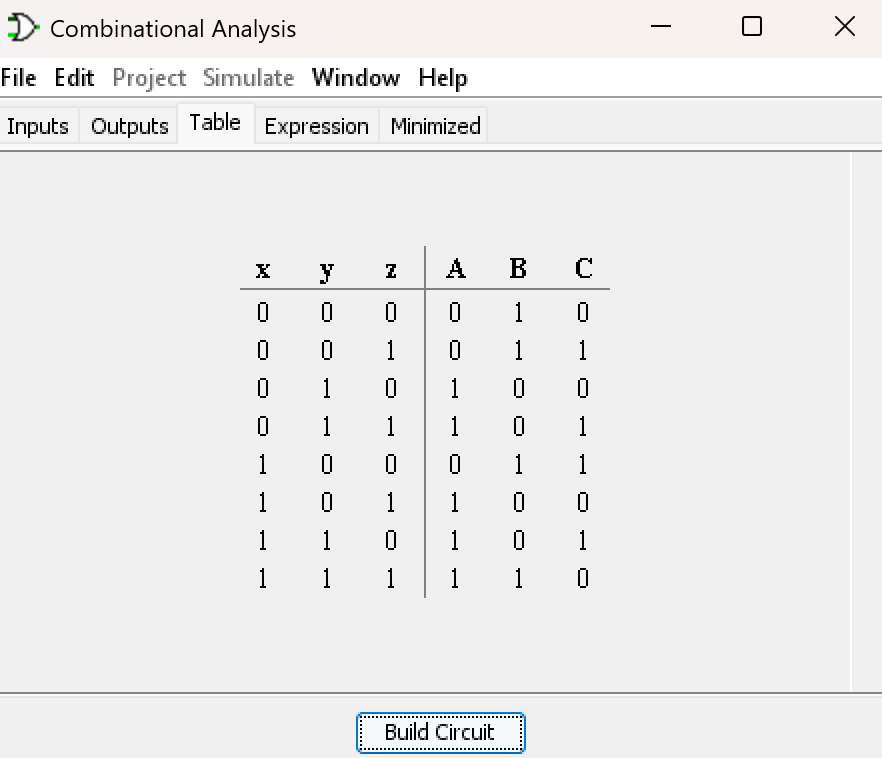
\includegraphics[width=\textwidth]{./img/table.png} 
     \end{figure}
}

\end{document}